%TODO @Konne,Jeff

\section{Starten der Applikation}
\label{sec:5:startapp}
\begin{figure}[H]
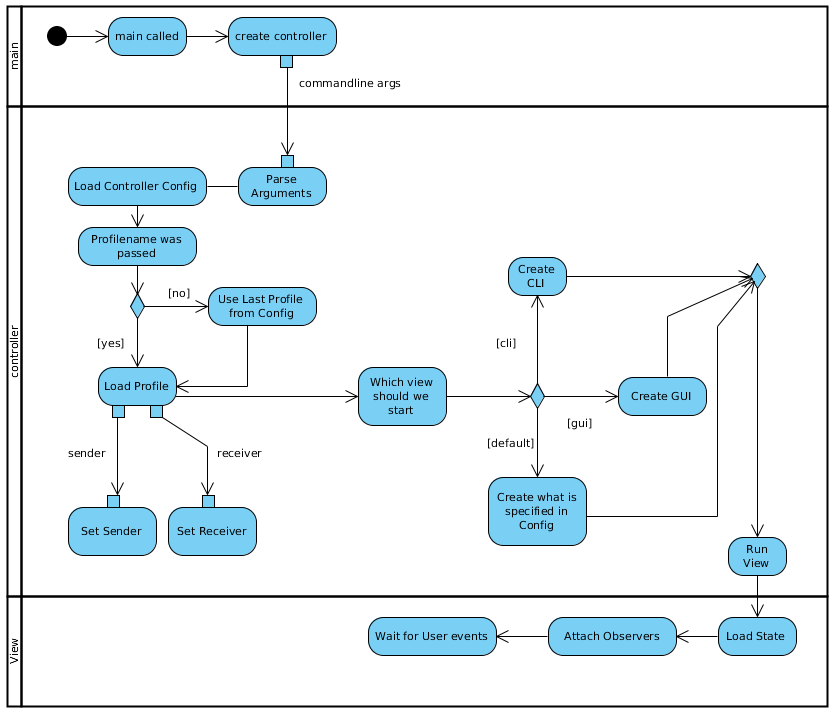
\includegraphics[width=15cm]{images/Init.png}
\centering
\caption{Starten der Applikation - UML Activity Diagramm}
\label{fig_init}
\end{figure}

Zeigt die Initialisierung der Applikation. Hierzu gehört das Parsen der
übergebenen Argumente, das Laden eines Profils und die Erstellung und 
Ausführung einer View.

\section{Beenden der Applikation}
\label{sec:5:stopapp}
\begin{figure}[H]
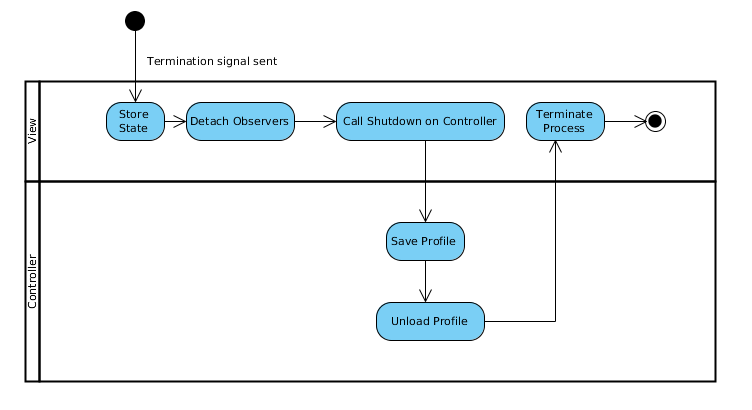
\includegraphics[width=15cm]{images/Shutdown.png}
\centering
\caption{Beenden der Applikation - UML Activity Diagramm}
\label{fig_shutdown}
\end{figure}

Zeigt wie die Applikation zu beenden ist, so dass sie sich auch danach
noch in einem konsistenten Zustand befindet.

\section{Profil Laden}
\label{sec:5:loadprofile}
\begin{figure}[H]
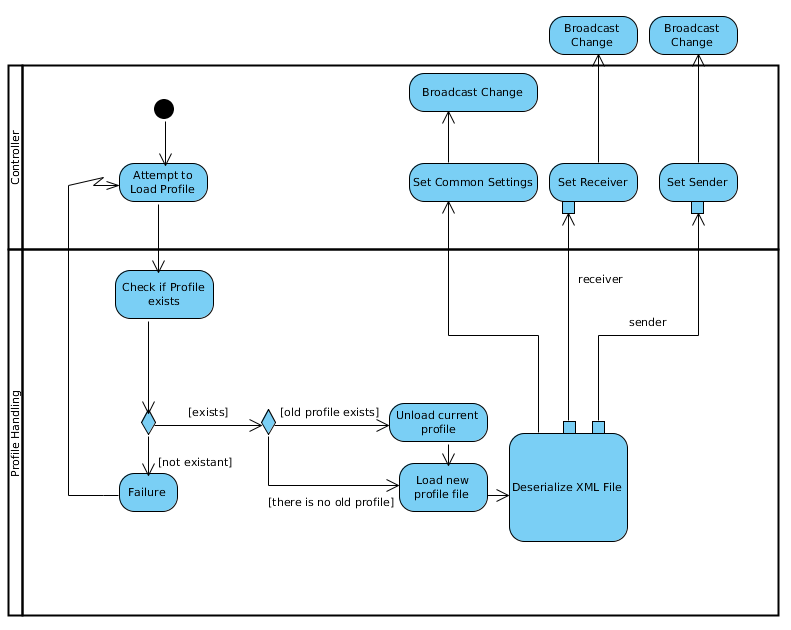
\includegraphics[width=15cm]{images/LoadProfile.png}
\centering
\caption{Profil Laden - UML Activity Diagramm}
\label{fig_loadprofile}
\end{figure}

Zeigt wie ein Profil geladen wird. Dies geschieht zum Beispiel beim
Start der Applikation und nach dem schließen eines anderen Profils.
Nach der Deserialisierung wird das System über die Änderungen im Profil
informiert.

\section{Profil Speichern}
\label{sec:5:loadprofile}
\begin{figure}[H]
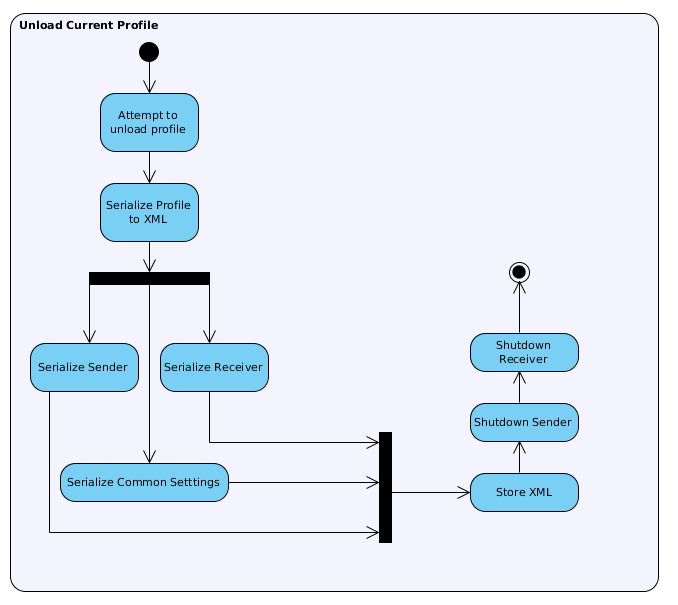
\includegraphics[width=15cm]{images/UnloadProfile.png}
\centering
\caption{Profil Speichern - UML Activity Diagramm}
\label{fig_unloadprofile}
\end{figure}

Bei der Speicherung und dem Schließen eines Profils werden alle 
wichtigen Komponenten serialisiert und danach heruntergefahren.

\section{Empfang eines Multicast-Pakets}
\label{sec:5:recmc}
\begin{figure}[H]
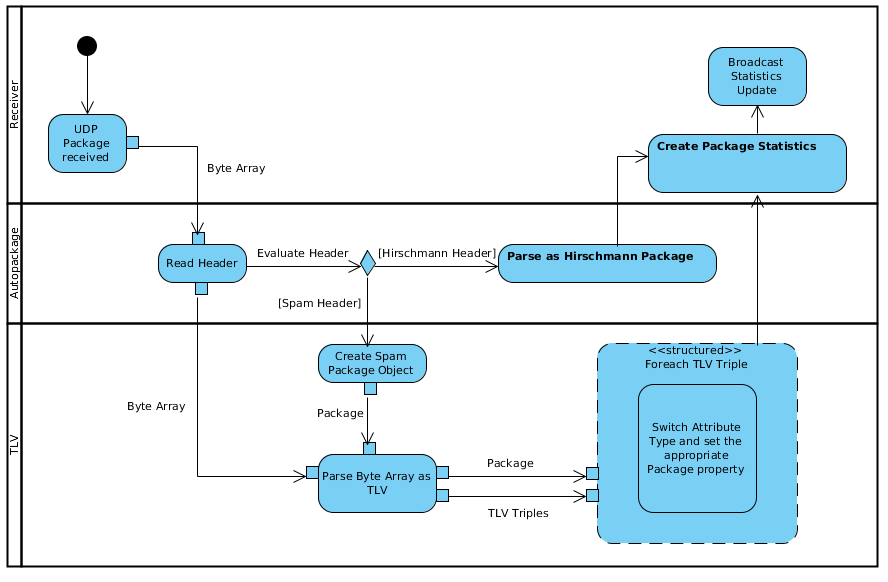
\includegraphics[width=15cm]{images/Receive.png}
\centering
\caption{Empfang eines Mutlicast-Pakets - UML Activity Diagramm}
\label{fig_receive}
\end{figure}

Hier wird beschrieben wie ein Spam Multicast Paket empfangen und
dann in ein Objekt umgewandelt wird.

\section{Automat der Empfangseinheit}
\label{sec:5:recmc}
\begin{figure}[H]
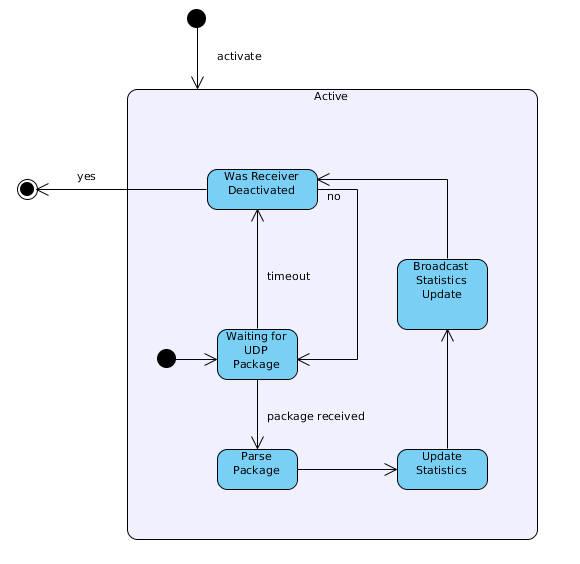
\includegraphics[width=15cm]{images/ReceiveState.png}
\centering
\caption{Automat der Empfangseinheit - UML Automat}
\label{fig_rcvstate}
\end{figure}

Dieser Automat beschreibt wie die Empfangskomponente auf das Empfangen
von Paketen wartet.

\section{Interaktion zwischen View, Sender und Empfänger}
\label{sec:5:readconf}
\begin{figure}[H]
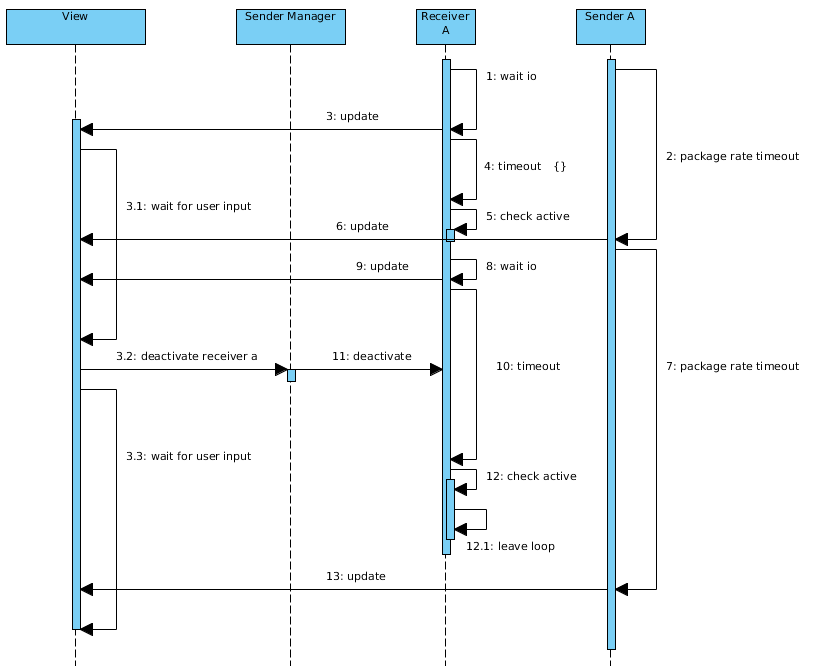
\includegraphics[width=15cm]{images/Threads.png}
\centering
\caption{Interaktion zwischen View, Sender und Empfänger - UML Sequence Diagramm}
\label{fig_threads}
\end{figure}

Dieses Sequenzdiagramm zeigt die Interaktion zwischen einer View und
dem Sender und Receiver. Hiermit wird die Observerstruktur und die
Nebenläufigkeit der einzelnen Komponenten veranschaulicht.
